\documentclass[10pt]{article}
\usepackage{icmlko}

\icmlmeta{IP 파운데이션 월드모델}{285}{진짜인데 안 보인다}{시장팝업의 범주 축을 넣었다 --- 신호는 유보에서 그대로 재현되는데 모형의 이득은 검출 문턱 아래다}

\begin{document}

\twocolumn[
\icmlheader

\begin{abstract}
노트 284가 시장팝업을 열면서 ``활성 축이 23 중 넷이라 굶었다''로 끝났다.
제일 센 신호였던 \texttt{category} 를 전용 축으로 넣었다(\texttt{mkt\_cat},
집단 크기 순 0$\sim$1 · 15건 미만 마스크 0 · 라벨 안 봄). 활성 축 4 $\to$ 5.
결과: 판 0.4713 $\to$ 0.4733($+$0.0021), \textbf{시장팝업 0.1970 $\to$
0.2137($+$0.0167)}, 진짜 0개(t 문턱 2.81). \textbf{방향은 맞는데 못 잰다} ---
시장팝업의 짝SE 가 0.0185 라 검출 문턱이 0.037 이고 관측이 그 절반이다
(노트 274의 법칙). \textbf{그리고 재는 김에 내 채택 근거가 엿보기였다는 걸
찾았다.} 노트 283이 보고한 \texttt{category} 의 크루스칼 $H{=}29.4$ 는
\textbf{205행 전부}로 잰 것이라 유보가 섞여 있다. 노트 239의 규약은 ``채택
근거는 학습 구간''이다. 학습 101행만으로 재면 \textbf{$H{=}14.5$
($p{=}0.0128$)} --- \textbf{절반이다.} 다만 여기서 좋은 소식이 나온다:
유보 104행만으로 재도 \textbf{$H{=}14.4$} 이고 집단 중앙값의 순위상관이
\textbf{$+$0.943}($p{=}0.005$)이다. \textbf{신호는 진짜고 재현된다 --- 내가
보고한 세기가 부풀어 있었을 뿐이다.} 두 구간이 거의 같은 $H$ 를 내는데 합치면
29.7 이 되는 것은 $n$ 이 두 배라서다. 그래서 이 노트의 결론은 둘이다.
\textbf{①} 축은 남긴다 --- 학습 구간 근거가 있고(약하지만) 유보에서 재현되며
아무 도메인도 안 해쳤다. \textbf{②} 그런데 \textbf{이 도메인에서 $+$0.0167 을
확인하려면 유보가 네 배}(104 $\to$ 420행) 있어야 한다. 없다.
\end{abstract}
]

\section{굶은 도메인에 밥을 준다}

노트 284가 시장팝업(205행 · 학습 101 · 유보 104)을 열고 $\rho{=}0.197$ 을
받았다. 원인은 축이었다 --- 활성 축이 23 중 \textbf{넷}이고 나머지 열 도메인은
13$\sim$19다. 검색 · 위키 · 달력 · 태그가 전부 마스크 0 이다.

노트 283이 잰 신호 중 제일 센 것이 \texttt{category} 였다. 넣었다.

\begin{center}\small
\begin{tabular}{ll}
\hline
\texttt{mkt\_cat} & \\
\hline
눈금 & 집단을 크기 순으로 0$\sim$1(\texttt{grpaxes} 관례) \\
문턱 & 15건 미만은 마스크 0 --- 일곱 집단이 194/205 \\
라벨 & \textbf{한 번도 안 본다}(집단 크기만 쓴다) \\
이름 & \textbf{전용} --- 학습 101행이라 청력 문턱 22 위 \\
\hline
\end{tabular}
\end{center}

전용 이름을 준 근거가 노트 281이다. 노트 283이 ``얇은 도메인은 공유 축에
태워라''고 적었는데 그건 \emph{학습행이 청력 문턱 아래일 때}의 규약이다.
시장팝업은 101행이라 해당 없다.

\section{방향은 맞는데 못 잰다}

\begin{figure*}[t]
\centering
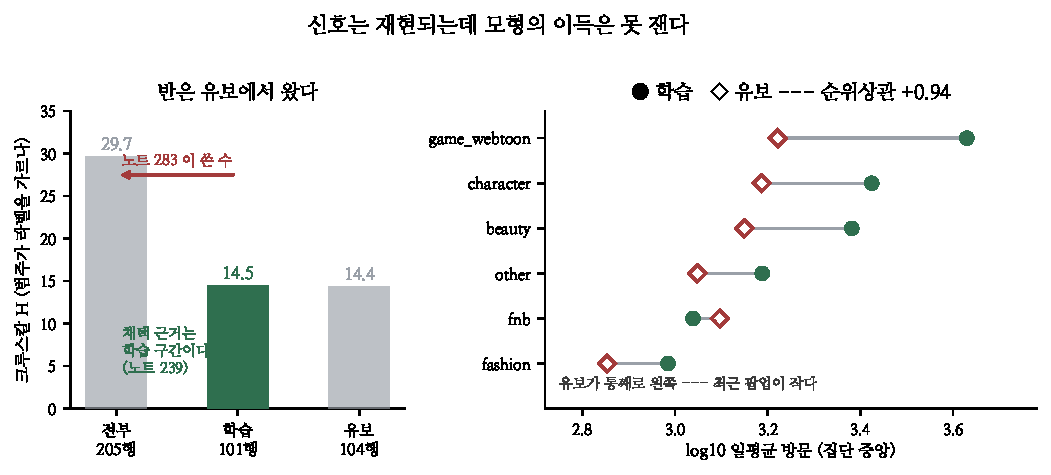
\includegraphics[width=\textwidth]{figs/unseen.pdf}
\caption{왼쪽 --- 구간별 크루스칼 $H$. 오른쪽 --- 집단 중앙값이 학습과 유보에서
어디에 있나. 유보가 통째로 왼쪽인 것은 최근 팝업이 작기 때문이다(0.69배).}
\end{figure*}

\begin{center}\small
\begin{tabular}{lrrr}
\hline
도메인 & 전 & 후 & 차 \\
\hline
아이돌 & 0.1085 & 0.1519 & $+$0.0434 ($t{=}1.31$) \\
\textbf{시장팝업} & 0.1970 & 0.2137 & \textbf{$+$0.0167} ($t{=}0.91$) \\
게임 & 0.6240 & 0.6290 & $+$0.0050 ($t{=}1.48$) \\
애니 & 0.4993 & 0.5030 & $+$0.0036 ($t{=}2.62$) \\
$\cdots$ & & & \\
펀딩 & 0.2350 & 0.2321 & $-$0.0029 ($t{=}{-}0.32$) \\
\hline
\multicolumn{4}{l}{판 $+$0.0021 · \textbf{진짜 0개} (t 문턱 2.81)} \\
\hline
\end{tabular}
\end{center}

\textbf{시장팝업이 $+$0.0167 로 예측한 방향으로 움직인다.} 그런데 짝SE 가
0.0185 라 $t{=}0.91$ 이다. 노트 274의 법칙으로 이 도메인의 검출 문턱은
$2{\times}0.0185 = 0.037$ 이고 \textbf{관측은 그 절반}이다. \emph{못 잰다.}

\paragraph{씨앗을 늘려도 안 된다} 이 SE 는 유보 행의 붓스트랩이지 씨앗 분산이
아니다. 아이돌에서와 같다(노트 282) --- \textbf{한계는 표본이지 씨앗이
아니다.} $+$0.0167 을 문턱 위로 올리려면 유보가 \textbf{네 배}(104 $\to$
420행) 있어야 한다.

\paragraph{덤} 마스크 0 인 아이돌이 $+$0.0434 로 제일 크게 움직였다. 노트
259의 자리바꿈이 이번엔 \emph{양수} 쪽으로 났다. 유의하지 않다($t{=}1.31$).

\section{그런데 채택 근거가 엿보기였다}

재는 김에 노트 283이 보고한 수를 다시 봤다.

\begin{center}\small
\begin{tabular}{lrrl}
\hline
잰 구간 & $n$ & $H$ & $p$ \\
\hline
\textbf{전부}(노트 283) & 205 & \textbf{29.7} & $<$0.0001 \\
\textbf{학습만} & 101 & \textbf{14.5} & 0.0128 \\
유보만 & 104 & 14.4 & 0.0256 \\
\hline
\end{tabular}
\end{center}

\textbf{노트 283의 $H{=}29.4$ 는 유보를 포함해 잰 것이다.} 노트 239가 세운
규약이 ``채택 근거는 학습 구간이다''인데, 새 도메인을 조사하면서 그 규약을
안 걸었다. \textbf{정당한 근거는 $H{=}14.5$ 로 절반이고 $p$ 도 0.0128 이라
0.01 선 위다.}

\paragraph{그래도 신호는 진짜다} 여기서 좋은 쪽이 나온다. \textbf{유보만으로
재도 $H{=}14.4$ 로 거의 같고}, 집단 중앙값의 순위상관이 \textbf{$+$0.943}
($p{=}0.005$)이다.

\begin{center}\small
\begin{tabular}{ll}
\hline
학습 순서 & gw · character · beauty · other · fnb · fashion \\
유보 순서 & gw · character · beauty · \textbf{fnb · other} · fashion \\
\hline
\end{tabular}
\end{center}

여섯 중 다섯이 제자리고 뒤바뀐 한 쌍(\texttt{fnb}/\texttt{other})은 학습에서
0.15, 유보에서 0.05 차이라 사실상 동점이다. \textbf{합쳐서 29.7 이 되는 것은
효과가 커서가 아니라 $n$ 이 두 배라서다} --- 두 구간이 같은 $H$ 를 낸다는 게
그 증거다.

\paragraph{수준은 이동한다} 유보 집단 중앙값이 통째로 왼쪽이다(학습 3.285
$\to$ 유보 3.123, \textbf{0.69배}). 최근 팝업이 작다 --- 노트 283이 잰 연도
상관 $-$0.147 과 같은 것이다. \textbf{순서는 재현되고 수준은 이동한다} ---
순위 목표에는 앞쪽만 필요하다.

\section{둘로 나눠 결론}

\textbf{① 축은 남긴다.} 학습 구간 근거가 있고(약하지만 $p{=}0.0128$), 유보에서
순서가 재현되고($+$0.943), 어느 도메인도 안 해쳤다(진짜 0개). 라벨을 안 보고
만든 축이라 엿보기도 없다.

\textbf{② 그런데 이득을 확인할 방법이 지금 없다.} $+$0.0167 은 이 도메인의
검출 문턱 0.037 의 절반이다. \textbf{``축이 도움이 된다''와 ``도움을 잰다''는
다른 일}이고, 후자는 유보 420행이 필요하다.

이게 이 실험실이 오늘 하루 종일 만난 모양의 또 한 번이다 --- 노트 274가
``작은 도메인의 개선은 판이 못 본다''를 세웠고, 노트 282가 아이돌
$+$0.0651 에서, 여기서 시장팝업 $+$0.0167 에서 같은 벽을 만난다.
\textbf{새 도메인을 열어도 그 도메인이 작으면 벽은 따라온다.}

\paragraph{남은 것}
\begin{center}\small
\begin{tabular}{ll}
\hline
갈래 & 왜 \\
\hline
검색 · 위키 채우기 & 축 5 $\to$ 11$+$. 이게 제일 크다 \\
시장 레코드 더 & 유보 420행이면 $+$0.0167 을 잰다 \\
멀티 · IP 이력 축 & 이미 공유 축에 태웠는데 따로도? \\
학습 구간 재검사 & 다른 새 축들도 전부로 쟀나 \\
\hline
\end{tabular}
\end{center}

\paragraph{규약} \textbf{새 도메인을 조사할 때도 채택 검사는 학습 구간에서
한다.} 노트 239가 축에 대해 세운 규약인데 도메인 조사에는 안 걸고 있었다 ---
$H$ 가 절반으로 줄었다. 그리고 \textbf{두 구간에서 따로 재서 같은 값이 나오면
합친 수를 보고하지 않는다} --- 합치면 $n$ 이 커져 유의성이 부풀 뿐, 효과가
커지는 게 아니다.

\end{document}
